\begin{SingleSpace}
\chapter{Wave-Mean Flow Interactions in a Linear Theory of Tidally Locked Atmospheres}\label{ch:wave-mean-flow}
\vspace{0.5cm}
\chapterprecishere{``One might as well approximate the derivatives well instead of badly''\par\raggedleft--- \textup{John P. Boyd}, Chebyshev and Fourier Spectral Methods}
\end{SingleSpace}
\vspace{0.5cm}

%0 -- LEAD-IN PARAGRAPHS

%START ELEMENT
Tidally locked planetary atmospheres have such a different spatial energy input to planets like the Earth that it is not obvious that conventional Earth-like atmospheric dynamics should be able to describe them. However, the planetary-scale day-night forcing difference makes the global circulation highly susceptible to a simple shallow-water model, compared to the higher order effects controlling the Earth's atmosphere.

%FRAMING TEXT
This chapter discusses my work using a single-layer linear shallow-water model to investigate the global circulation of tidally locked planets. It follows directly from the work of XX and XX.

%SIGNPOSTS
After introducing the linear shallow-water model and the work of Matsuno, Gill, Showman, and Tsai, I will show how I linearised the model about a zonally uniform jet $\bar{U}(y)$ with latitudinal shear, as well as its associated geostrophic height perturbation $\bar{H}(y)$

A formula:
\[
  \underbrace{\frac{\sin^{2}\vartheta}{\Theta_{lm}(\vartheta)}\left(\frac{\partial^{2}}{\partial\vartheta^{2}}+\frac{\cos\vartheta}{\sin\vartheta}\frac{\partial}{\partial\vartheta}\right)\Theta_{lm}(\vartheta)+\sin^{2}(\vartheta)(l(l+1))}_{m^{2}}=\underbrace{-\frac{1}{\Phi_{m}(\varphi)}\frac{\partial^{2}}{\partial\varphi^{2}}\Phi_{m}(\varphi)}_{m^{2}}
\]

and another one:
\[
  P_l (x)\equiv\frac {1}{2^l}\sum_{k=0}^{\lfloor l/2\rfloor} (-1)^k \frac{(2l-2k)!}{k!(l-k)!(l-2k)!} x^{l-2k}
\]

%SUMMARISE CONCLUSIONS
I will show that linearising the jet about the shear flow and its height perurbation makes the forced linear response match nonlinear GCM simulations much more closely. The new model reveals scaling relations between the planetary parameters such as forcing strength, and the observable quantities such as the eastward hot-spot shift.


%SECTION 1 -- LINEAR SHALLOW-WATER AND UNIFORM FLOW
\section{The Shallow-Water Equations}

%SUBSECTION -- LINEAR SHALLOW-WATER
\subsection*{A Linear, Single-Layer Beta-Plane System}

We used the linear shallow-water equations on a one-layer equatorial beta-plane to model the atmosphere of a tidally locked planet. These equations describe the motion of a single layer of fluid of constant density where the horizontal scale of its flow is much greater than the depth of the fluid. The linear form of these equations describe small perturbations to this layer \citep{vallis2006book}. We model the atmosphere of a tidally locked planet with a similar shallow-water model to \citet{showman2011superrotation}. The model corresponds to an active upper layer following the single-layer shallow water equations, above a quiescent layer which can transport mass and momentum to and from the upper layer. The forcing due to stellar heating is represented by $Q$, a relaxation to the radiative equilibrium height field.

In this section, we derive the wave response to stationary forcing on the beta-plane \citep{matsuno1966quasi}. The beta-plane system approximates the Coriolis parameter as linear, which is only accurate at low latitudes but leads to more intuitive and useful solutions than the full spherical geometry. We solve the equations in a spherical geometry in Section \ref{sec:sphere-solutions}, and show that the beta-plane approximation leads to very similar solutions, as in other studies of the atmospheres of tidally locked planets \citep{showman2011superrotation} \citep{heng2014analytical}.

All the quantities are linearized as the sum of a zonally mean background value $F(y)$  and a perturbation with the form  $f(y) e^{i( k_{x} x-\omega t)}$ (unlike \citet{matsuno1966quasi}, who uses the less conventional form  $f(y) e^{i( k_{x} x+\omega t)}$). Throughout this paper, we will use capital letters for mean zonal quantities such as $\bar{U}$ and $\bar{H}$, and lower-case letters for perturbations to this background, such as $u$ and $h$ (unless otherwise specified, such as the forcing $Q$). The shallow-water equations for these perturbations with zero background flow are:

\begin{equation}\label{eqn:sw-eqns-1}
  \begin{gathered}
     \frac{\partial u}{\partial t} - \beta y v +\frac{\partial h}{\partial x} = 0 \\
      \frac{\partial v}{\partial t} + \beta y u + \frac{\partial h}{\partial y} = 0 \\
    \frac{\partial h}{\partial t} +c^{2}(\frac{\partial u}{\partial x} + \frac{\partial v}{\partial y}) = 0 \\
  \end{gathered}
\end{equation}

where $h$ is the height, $c = \sqrt{gH}$ is the gravity wave speed \citep{matsuno1966quasi}, and there is no friction or damping. Non-dimensionalizing with time scale $\sqrt{1/c \beta}$ and length scale $\sqrt{c/\beta}$ (the equatorial Rossby radius of deformation $L_{R}$), and assuming all quantities have the form $f(y) e^{i( k x-\omega t)}$, the free equations are:

\begin{equation}\label{eqn:sw-eqns-2}
  \begin{gathered}
      - i \omega u - y v + i k_{x} h = 0 \\
      - i \omega v + y u + \frac{\partial h}{\partial y} = 0 \\
      - i \omega h + i k u + \frac{\partial v}{\partial y} = 0 \\
  \end{gathered}
\end{equation}

%SUBSECTION -- ACCELERATION
\subsection*{Jet Acceleration}

%SUBSECTION -- UNIFORM FLOW
\subsection*{Wave Interactions with Uniform Flow}

%SECTION CONCLUSIONS

%SECTION 1 --
\section{Zonal Acceleration}

Chapter X showed that the global circulation and temperature distribution of an atmosphere on a tidally locked planet depends greatly on the zonal jets present on the planet.



%SUBSECTION --
\subsection*{Acceleration in a Matsuno-Gill Model}

The zonally averaged zonal momentum equation is:

\begin{equation}
  \frac { \partial \overline { u } } { \partial t } = \underbrace { \overline { v } ^ { * } \left[ f - \frac { \partial \overline { u } } { \partial y } \right] } _ { I } \underbrace { - \frac { 1 } { \overline { h } } \frac { \partial } { \partial y } \left[ \overline { ( h v ) ^ { \prime } u ^ { \prime } } \right] } _ { I I } + \underbrace { \left[ \frac { 1 } { \overline { h } } \overline { u ^ { \prime } Q ^ { \prime } } + \overline { R _ { u } } ^ { * } \right] } _ { I I I } \underbrace { - \frac { \overline { u } ^ { * } } { \tau _ { \mathrm { drag } } } } _ { I V } - \frac { 1 } { \overline { h } } \frac { \partial \left( \overline { h ^ { \prime } u ^ { \prime } } \right) } { \partial t }
\end{equation}

In the Matsuno-Gill model, this gives zero acceleration at the equator without R.

%SUBSECTION --
\subsection*{Vertical Momentum Transport}

%SUBSECTION --
\subsection*{Horizontal Momentum Transport from Stationary Waves}




%SECTION CONCLUSIONS


%SECTION 2 -- SHEAR FLOW ON BETA-PLANE AND SPHERICAL
\section{Wave Interactions with Shear Flow}


\begin{figure}
  \begin{subfigure}[b]{0.4\textwidth}
    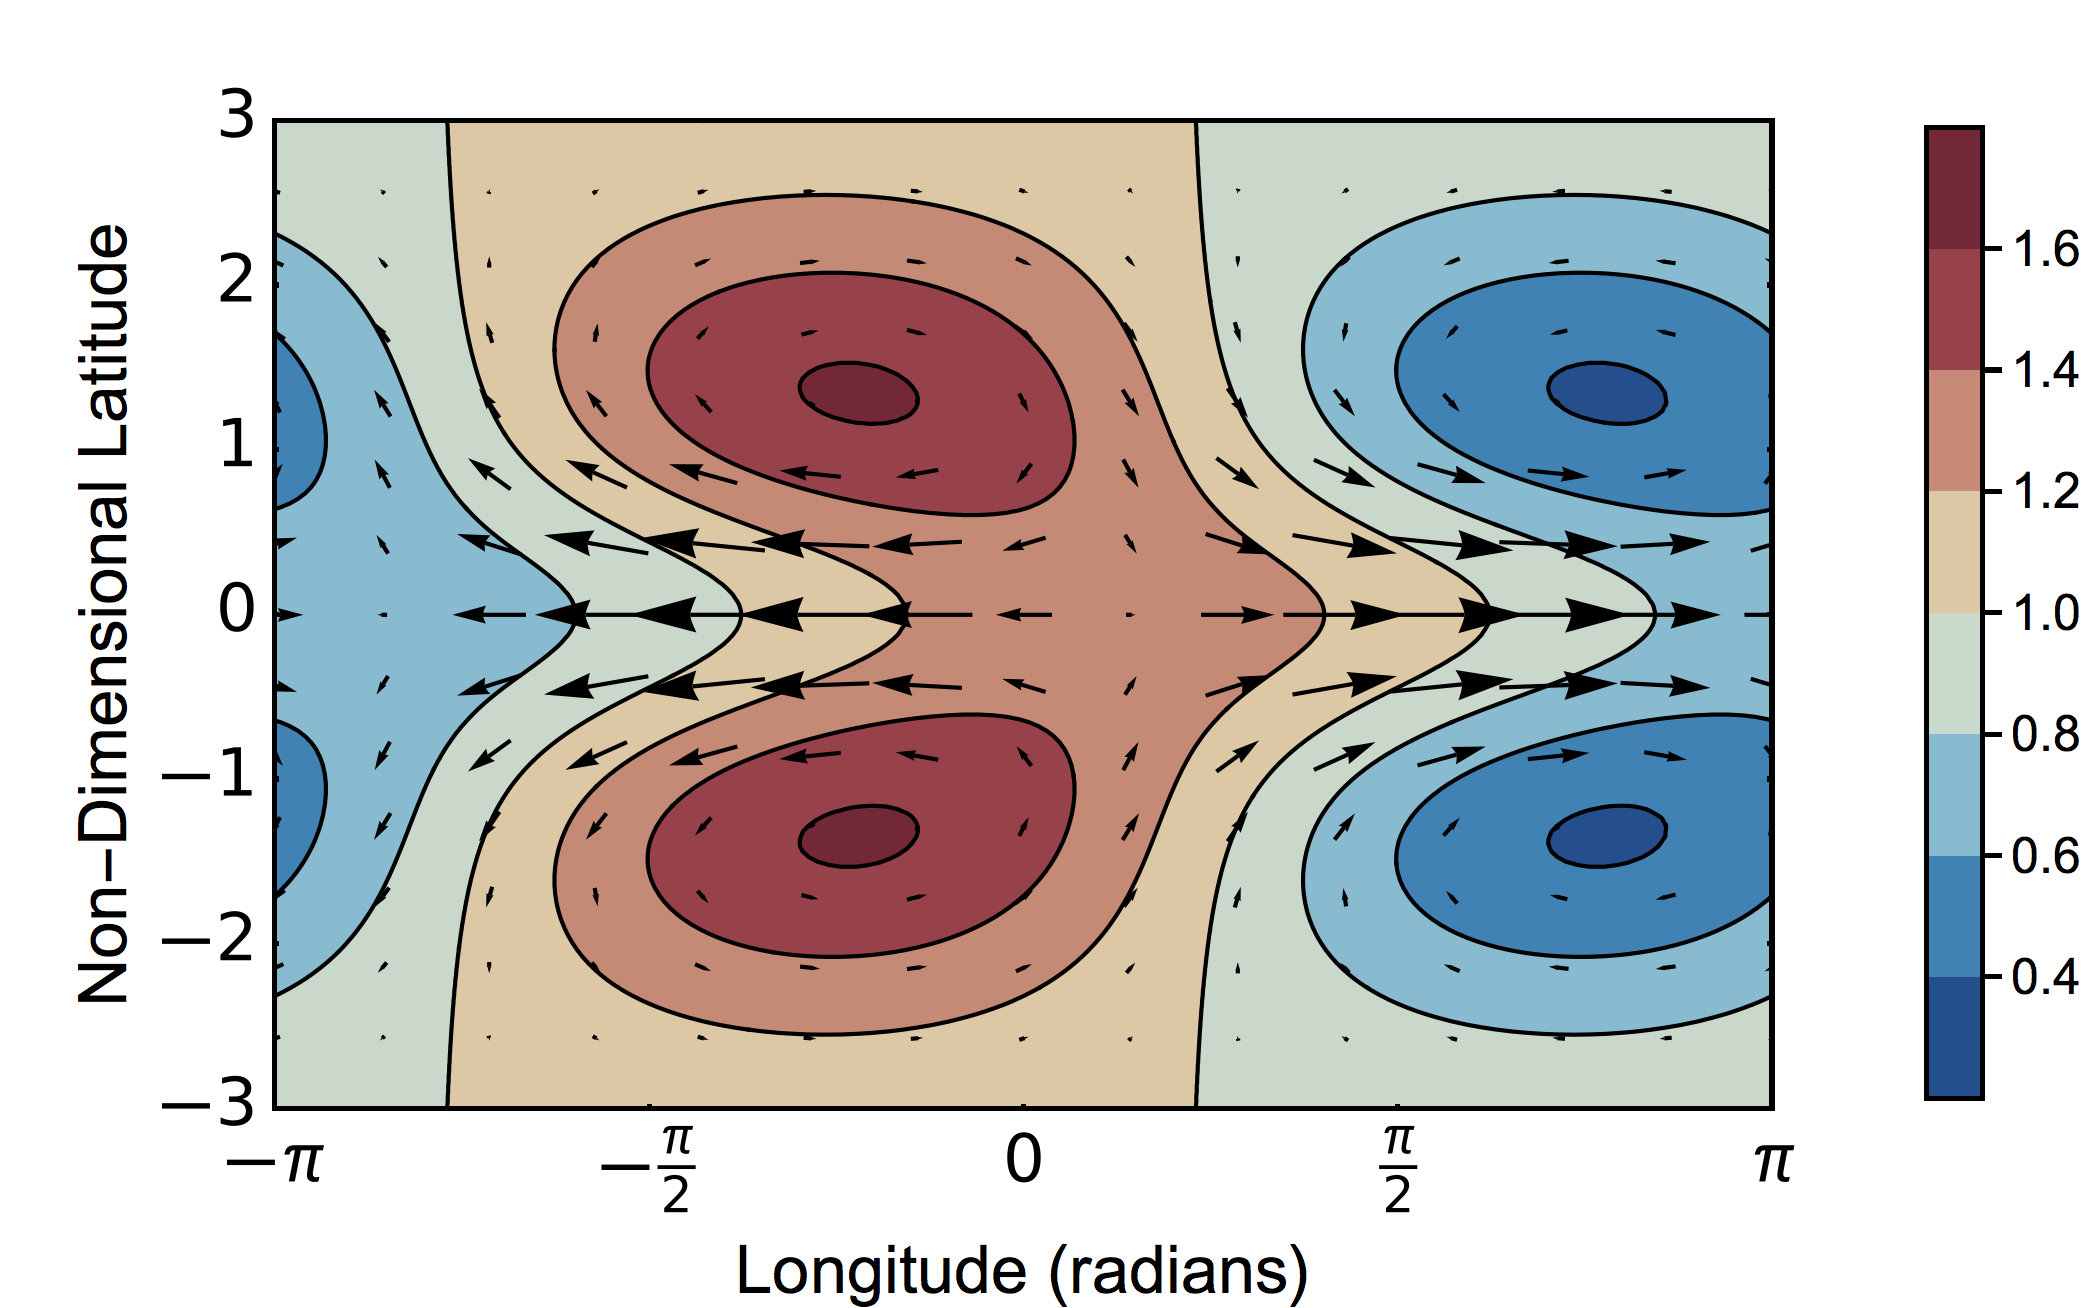
\includegraphics[width=\textwidth]{figures/wave-mean-flow/ps-no-flow.png}
    \caption{Zero Flow.}
    \label{fig:ps-no-flow}
  \end{subfigure}
  %
  \begin{subfigure}[b]{0.4\textwidth}
    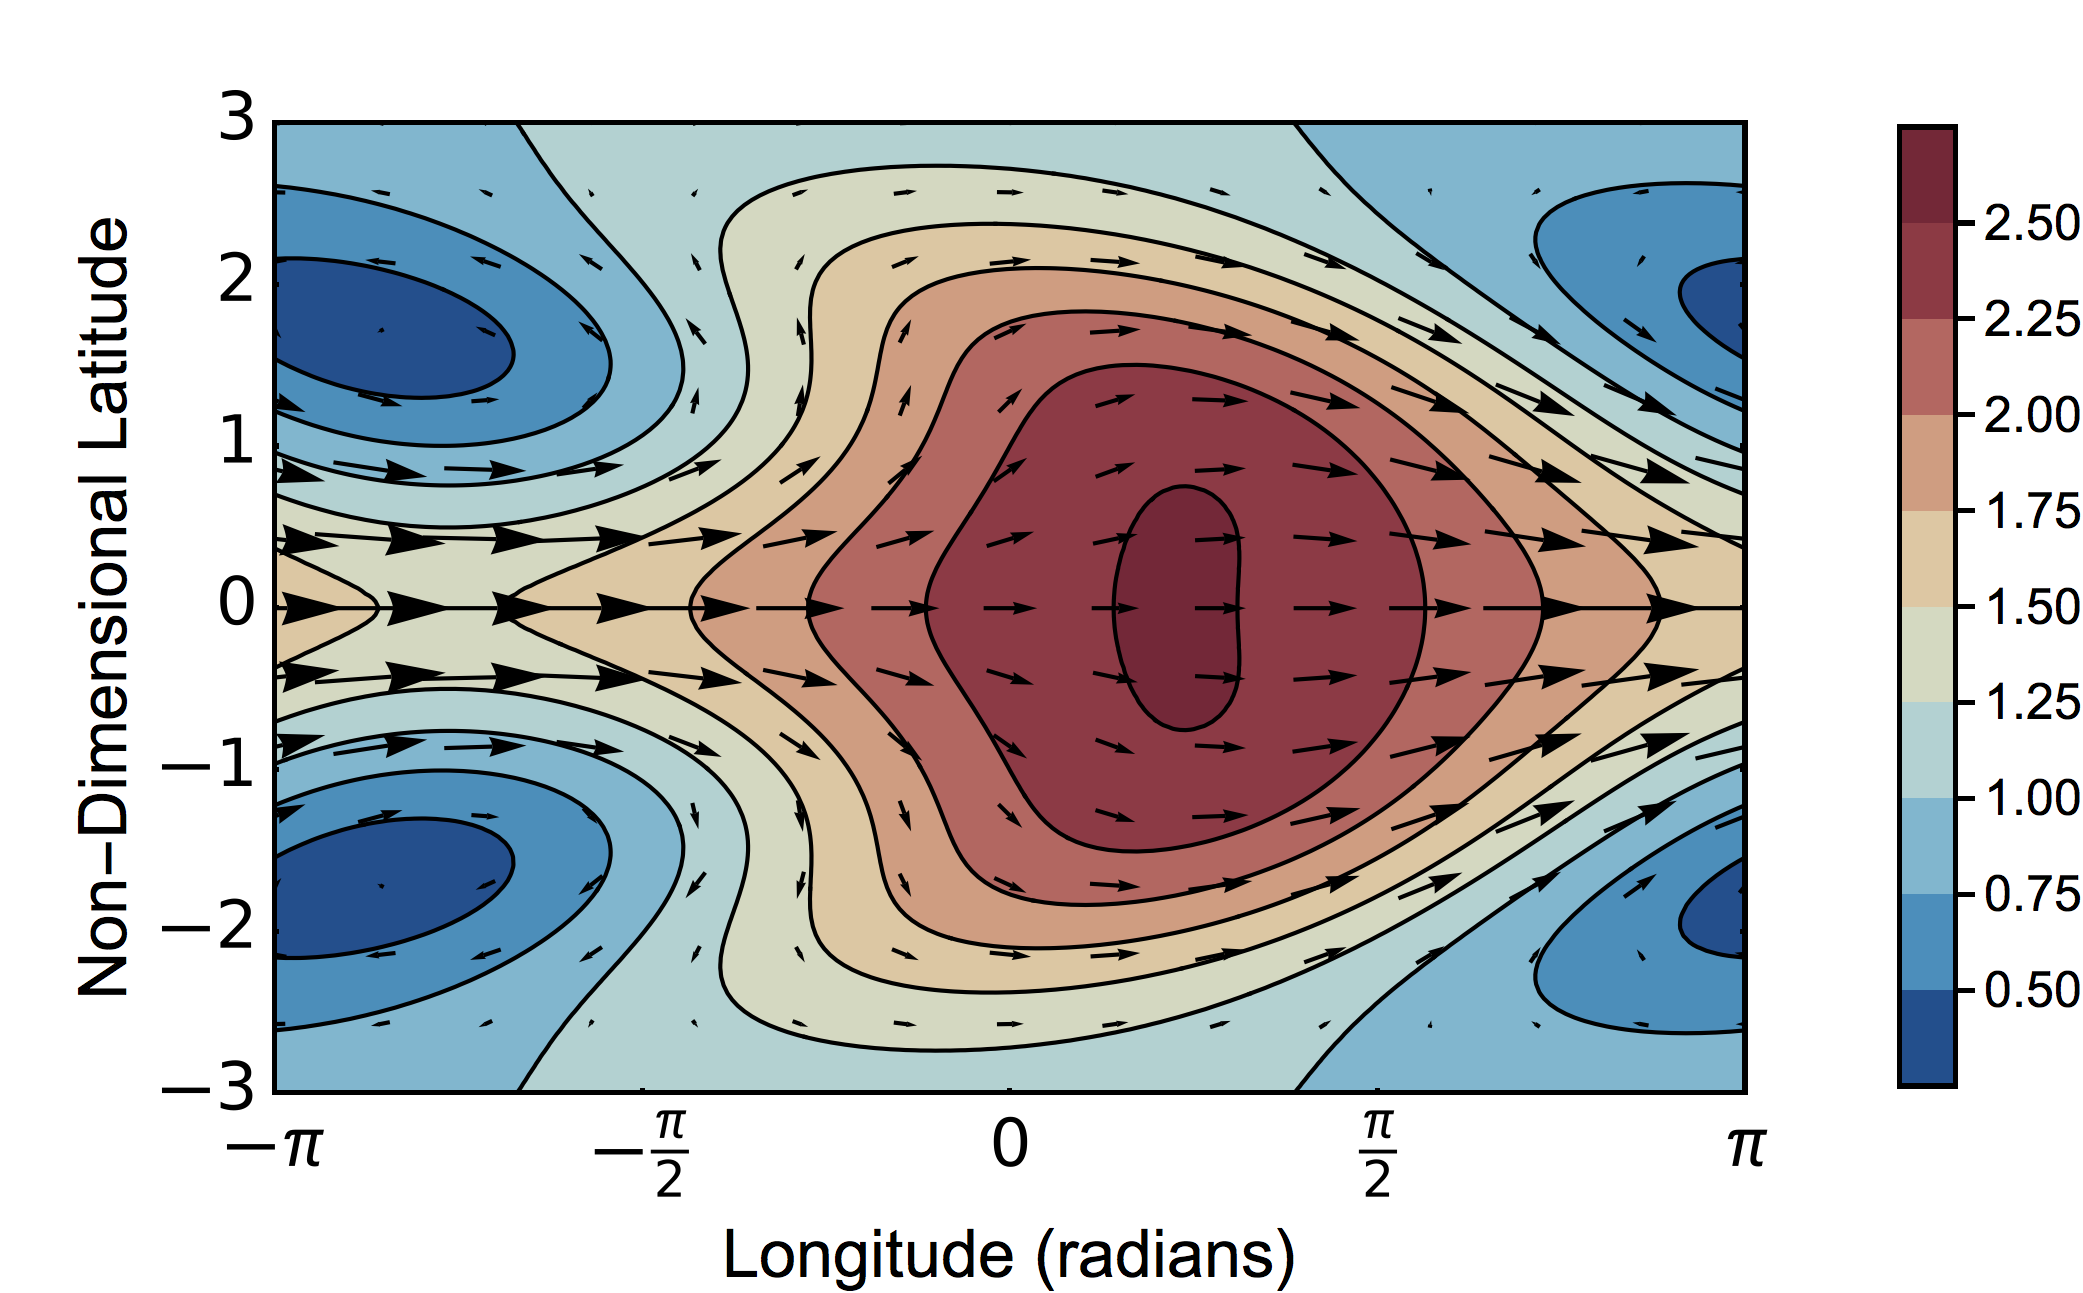
\includegraphics[width=\textwidth]{figures/wave-mean-flow/ps-shear-flow.png}
    \caption{Shear Flow.}
    \label{fig:ps-shear-flow}
  \end{subfigure}
  \caption{Zero Flow and Shear Flow.}
  \label{fig:ps-flow}
\end{figure}


%SUBSECTION -- BETA-PLANE
\subsection*{Shear Flow on the Beta-Plane}

%SUBSECTION -- SPHERICAL
\subsection*{Shear Flow on a Sphere}

%SECTION CONCLUSIONS



%SECTION 3 -- SCALING RELATIONS
\section{Scaling Relations}

%SUBSECTION -- 1D SCALING
\subsection*{1D Scaling Relations}

%SUBSECTION -- 2D SCALING
\subsection*{2D Scaling Relations}

%SECTION CONCLUSIONS





%CONCLUSIONS

%RESTATE SECTION CONCLUSIONS

%OPEN OUT CONCLUSIONS



% \bibliographystyle{unsrtnat}
% \bibliography{../references.bib}
